\documentclass[10pt]{exam}
\usepackage[hon]{template-for-exam}
\usepackage{multirow}
\usepackage[table,dvipsnames]{xcolor}
\usepackage{pgf-pie}
\usepackage{wrapfig}
\usepackage{enumitem}
\usepackage{graphicx}
\graphicspath{{./images}}
\setlist[enumerate]{topsep=0pt,itemsep=-1ex,partopsep=1ex,parsep=1ex}
\usepackage[super]{nth}


\newcommand{\mg}{\rowcolor{Goldenrod}}


\title{Course Information Guide \\ Honors Physics}
\author{Rohrbach}


\begin{document}

\maketitle

\noindent Zachary J. Rohrbach, Instructor

\noindent (317) 544-5000

\noindent \texttt{ZJRohrbach@avon-schools.org}

\section*{Course Description}

Physics is the study of how the universe works on the most fundamental level.  In this 
class, you will use your powers of observation and logical as well as mathematical 
reasoning to describe, explain, and predict the behavior of objects.

\paragraph{Course Goals} 
As a result of taking Physics I, you will:

\begin{enumerate}
	\item Know and understand the process that is used to make the scientific discoveries that 
				are reported in the media or in the workplace
	\item Understand the scientific principles that underlie motion, forces, waves, and electricity.
	\item Apply your mathematical skills to solving real-world problems
	\item Develop problem solving and scientific literacy skills
\end{enumerate}


\section*{Required Materials}

You are expected to bring the following materials with you to class every day.  

\begin{center}

\begin{tikzpicture}
	
	
	\node [font=\large] at (0, .5) {Notebook};
	\node [font=\small\it] at (0, 0)  {(I recommend quad-ruled)};
	\node at (0,1.7) {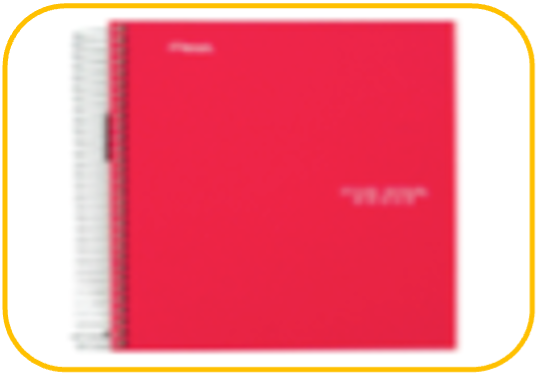
\includegraphics[width=2.4cm]{notebook}};


	\node [font=\large] at (3, .5) {School};
	\node [font=\large] at (3, 0)  {Laptop};
	\node at (3,1.7) {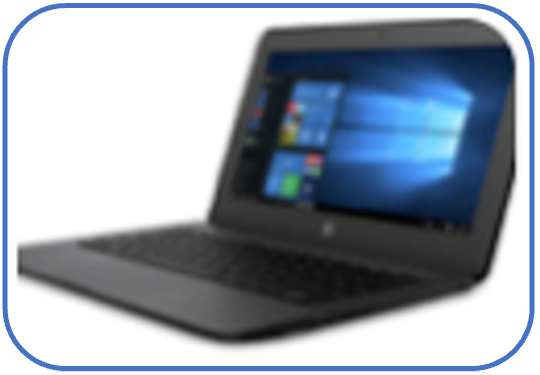
\includegraphics[width=2.4cm]{laptop}};

	
	\node [font=\large] at (6, .5) {Computer};
	\node [font=\large] at (6, 0)  {Charger};
	\node at (6,1.7) {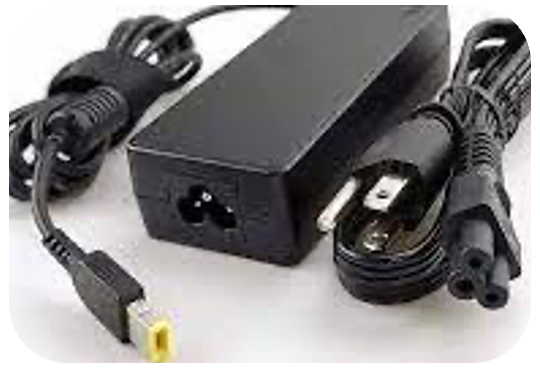
\includegraphics[width=2.4cm]{charger}};
	
	\node [font=\large] at (9, .5) {Student};
	\node [font=\large] at (9, 0) 	{Agenda};
	\node at (9,1.7) {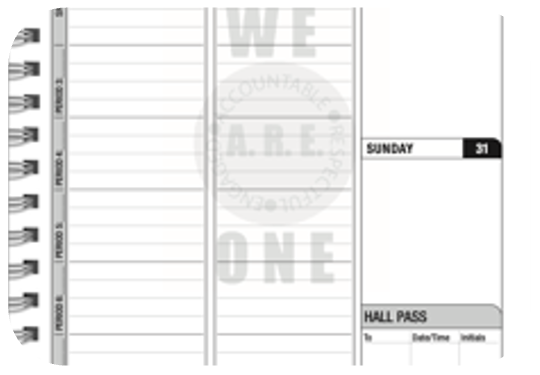
\includegraphics[width=2.4cm]{agenda}};

	\node [font=\large] at (12, .5) {Reading};
	\node [font=\large] at (12, 0)  {Book};
	\node at (12,1.7) {
\includegraphics[width=2.4cm]{book}};


\end{tikzpicture}

\end{center}

\paragraph{Notebook:}
	You should have a writing utensil and a spiral notebook that you bring with you every day.  I recommend that it be a quad-ruled (graphing) notebook.  We will use the notebook to take notes and work problems. 

\paragraph{Laptop and Charger:}
	Please bring your laptop and charger with you to class every day.  We will not use it every day or even most days, but there are certain assignment you will be unable to complete without it.	

\paragraph{Student Agenda:}
	This is required by school policy.  If you need to use the restroom, you must have your agenda.  I will write one restroom pass per week. 

\paragraph{Reading Book:}
	If there is downtime in class, you may not use your phone.  You may, however, read a book.




\section*{Methods of Evaluation}

Your pre-exam grade will be based on the methods of 
evaluation shown below. The weighting of each of these 
categories is subject to change. Your overall class 
grade will consist of the pre-exam grade (85\%) and the
final exam grade (15\%).

\begin{enumerate}
	\item	Homework (30\%)
	\begin{itemize}
		\item 
			Homework plays an important role in helping you understand the material.  Therefore, it is important that it gets done in a timely manner! 
		\item 
			At the beginning of each unit, all the problems of the unit will be given to you as a chapter syllabus.  
		\item 
			There will be one HW quiz each unit based upon the problems you were to complete on the syllabus. They are also open-note!  Therefore, it is to your advantage to bring to class your homework!
		\item 
			Homework is accepted for full credit until Test Day.  There will be a 50\% penalty for homework turned in after test day.  Homework will not be accepted any later than the Test for the following unit.
	\end{itemize}
	\item	Labs/Projects (30\%)
	\begin{itemize}
		\item 
			Many labs will have an associated worksheet to turn in or a short summary paragraph to complete via Schoology.  
		\item 
			A few labs will require a fully typed lab write-up to be uploaded to Schoology.
		\item 
			Late labs will be assessed a penalty of 10\% per school day (whether or not class meets) up to 50\%.  Labs that are more than a month late will not be accepted.
		\item 
			There will be one research project in the Spring Semester.  If you complete your research project late, it is immediately assessed a 50\% penalty.
	\end{itemize}
	\item	Tests (40\%)
	\begin{itemize}
		\item	
			Each chapter will end with a quiz or a test.
		\item 
			Tests may be corrected for half-credit back on missed questions.  In order to be eligible for test corrections, you must have no outstanding lab assignments and must have at least an 80\% on your homework score for that chapter.
	\end{itemize}
	
\end{enumerate}


\section*{Other Class Policies}

\paragraph{Tardies}
	My tardy policy is the same as the school's. You are tardy if you are not in the classroom by the time the bell rings.  If you do come in late, please sign the tardy log.

\paragraph{Cell Phones and Earbuds}
	In Honors Physics, there is no instructional need for cell phones or earbuds.  They should therefore be put away at all times.  Failure to comply will result in the progressive discipline outlined in the AHS Student Handbook.

\paragraph{Absences and Makeup Work}
	I will often post video explanations and recordings for students who are absent on Schoology.  If you are absent, it is your responsibility to check Schoology and contact me with any questions.

	There are some activities that we do in class which will not need to be made up.  Students with \emph{excused} absences will be exempted from these assignments in the grade book.  Students with \emph{unexcused} or \emph{unverified} absences will receive a zero, which cannot be made up.  This is in line with the policy in the AHS Student Handbook.




\end{document}